\PassOptionsToPackage{dvipsnames}{xcolor}
\documentclass[ignorenonframetext, hyperref=unicode,compress]{beamer}


\usepackage{cmap}
\usepackage[T2A]{fontenc}
\usepackage[utf8x]{inputenc}
\usepackage[bulgarian]{babel}
\selectlanguage{bulgarian}

\usepackage{graphicx}
\usepackage{listings}

\hypersetup{
	colorlinks=true,
	linkcolor=blue,
	filecolor=blue,
	urlcolor=blue,
	anchorcolor=blue,
	citecolor=blue
}

\lstset{language=java, 
  numbers=left, 
  numberstyle=\tiny,
  stepnumber=1, 
  numbersep=3pt, 
  tabsize=2, 
  texcl,
  basicstyle=\ttfamily\small,
  identifierstyle=\ttfamily\small,
  keywordstyle=\sffamily\bfseries\small,
  extendedchars=true, inputencoding=utf8x,
  backgroundcolor=\color[rgb]{1,1,0.845},
  escapeinside={/*@}{@*/}}

\newcommand{\Cpp}{{\ttfamily\bfseries C++}}
\newcommand{\CC}{{\ttfamily\bfseries C}}

% \usepackage{algpseudocode}

%\usepackage{ucs}

%\logo{\includegraphics[height=0.4cm]{../macros/logo_elsys.png}}

\titlegraphic{\href{http://creativecommons.org/licenses/by-sa/3.0/}{
\includegraphics{pics/cc.png}}}

\newcommand{\authors}{%
\author[Л.~Чорбаджиев]{Любомир Чорбаджиев}
\institute[ELSYS] {%
Технологично училище ``Електронни системи'' \\
Технически университет, София
}}

\usepackage{tikz}
\usetikzlibrary{arrows,shapes.misc,calc,backgrounds,fit,decorations.pathmorphing,positioning,chains,scopes,topaths,automata,shapes,trees}

\tikzset{obj/.style={rectangle,minimum size=6mm,
				very thick,draw=red!50!black!50,top color=white,bottom color=red!50!black!20, font=\ttfamily},
ref/.style={rectangle,
		minimum size=8mm,
		% The rest
		very thick,draw=black!50,
		top color=white,bottom color=black!20},
	every node/.style={font=\ttfamily},
	>=stealth',
	thick,
	draw=black!50,
	shorten >=1pt,node distance=2cm and 2.5cm,on grid}


\mode<article>
{

}

\mode<presentation>
{
  \usetheme[secheader=true]{Madrid}
  \usecolortheme{crane}
  \usefonttheme[onlylarge]{structurebold}
  \setbeamercovered{transparent}
}

\usepackage[unicode]{hyperref}

%%% Local Variables: 
%%% mode: latex
%%% TeX-master: t
%%% End: 


\title{Хеширане, колекции и компаратори}
\authors
\date{\today}

\usetikzlibrary{shapes}

\begin{document}

\frame{\titlepage}

\begin{frame}
\small
{\bf Забележка:} Тази лекция е адаптация на:
\begin{itemize}
  \item \href{http://ocw.mit.edu/NR/rdonlyres/Electrical-Engineering-and-Computer-Science/6-092January--IAP--2006/66BAC837-433E-48A5-BA15-B766E0B7CDEA/0/lecture3.pdf}{Scott Ostler: {\em Hashing, Collections, and Comparators}} from
\href{http://ocw.mit.edu/OcwWeb/Electrical-Engineering-and-Computer-Science/6-092January--IAP--2006/CourseHome/index.htm}{
{\em 6.092: Java for 6.170} (MIT OpenCourseWare:
Massachusetts Institute of Technology)}\\
{\bf Лиценз:}
\href{http://ocw.mit.edu/OcwWeb/web/terms/terms/index.htm\#cc}{Creative commons
BY-NC-SA}

\end{itemize}

\end{frame}
\begin{frame}
\frametitle{Съдържание}
\tableofcontents %[hideallsubsections]
\end{frame}


% \begin{frame}[containsverbatim]
% 	\begin{tikzpicture}[edge from parent fork down, level 1/.style={sibling distance=4cm,level distance=2.5cm},
%     level 2/.style={sibling distance=2cm, level distance=2.5cm}, 
% 	every node/.style={rectangle, shade, top color=white,
%     bottom color=blue!50!black!20, draw=blue!40!black!60, very thick,inner sep=2mm,rectangle split, rectangle split parts=2},edge from parent/.style={very thick,draw=blue!40!black!60,arrows=triangle 90-}]
% 		\node {\lstinline{root}}
% 		child {node {left}}
% 		child {node {right}
% 		child {node {child}}
% 		child {node {child}}
% 		};
% 	\end{tikzpicture}
% \end{frame}

\section{Хеширане}

\begin{frame}[containsverbatim]\frametitle{Хеширане}
\begin{itemize}
 \item Миналият път разгледахме как се предефинира (override) метода \lstinline{equals} на класа \lstinline{java.lang.Object}
 \item Днес ще разгледаме как се предефинира (override) метода \lstinline{hashCode}.
 \item Целта е да разберем защо това е необходимо и как се прави.
\end{itemize}
\end{frame}

\begin{frame}[containsverbatim]\frametitle{Хеширане}
\begin{figure}[h]
\center
\scalebox{0.4}{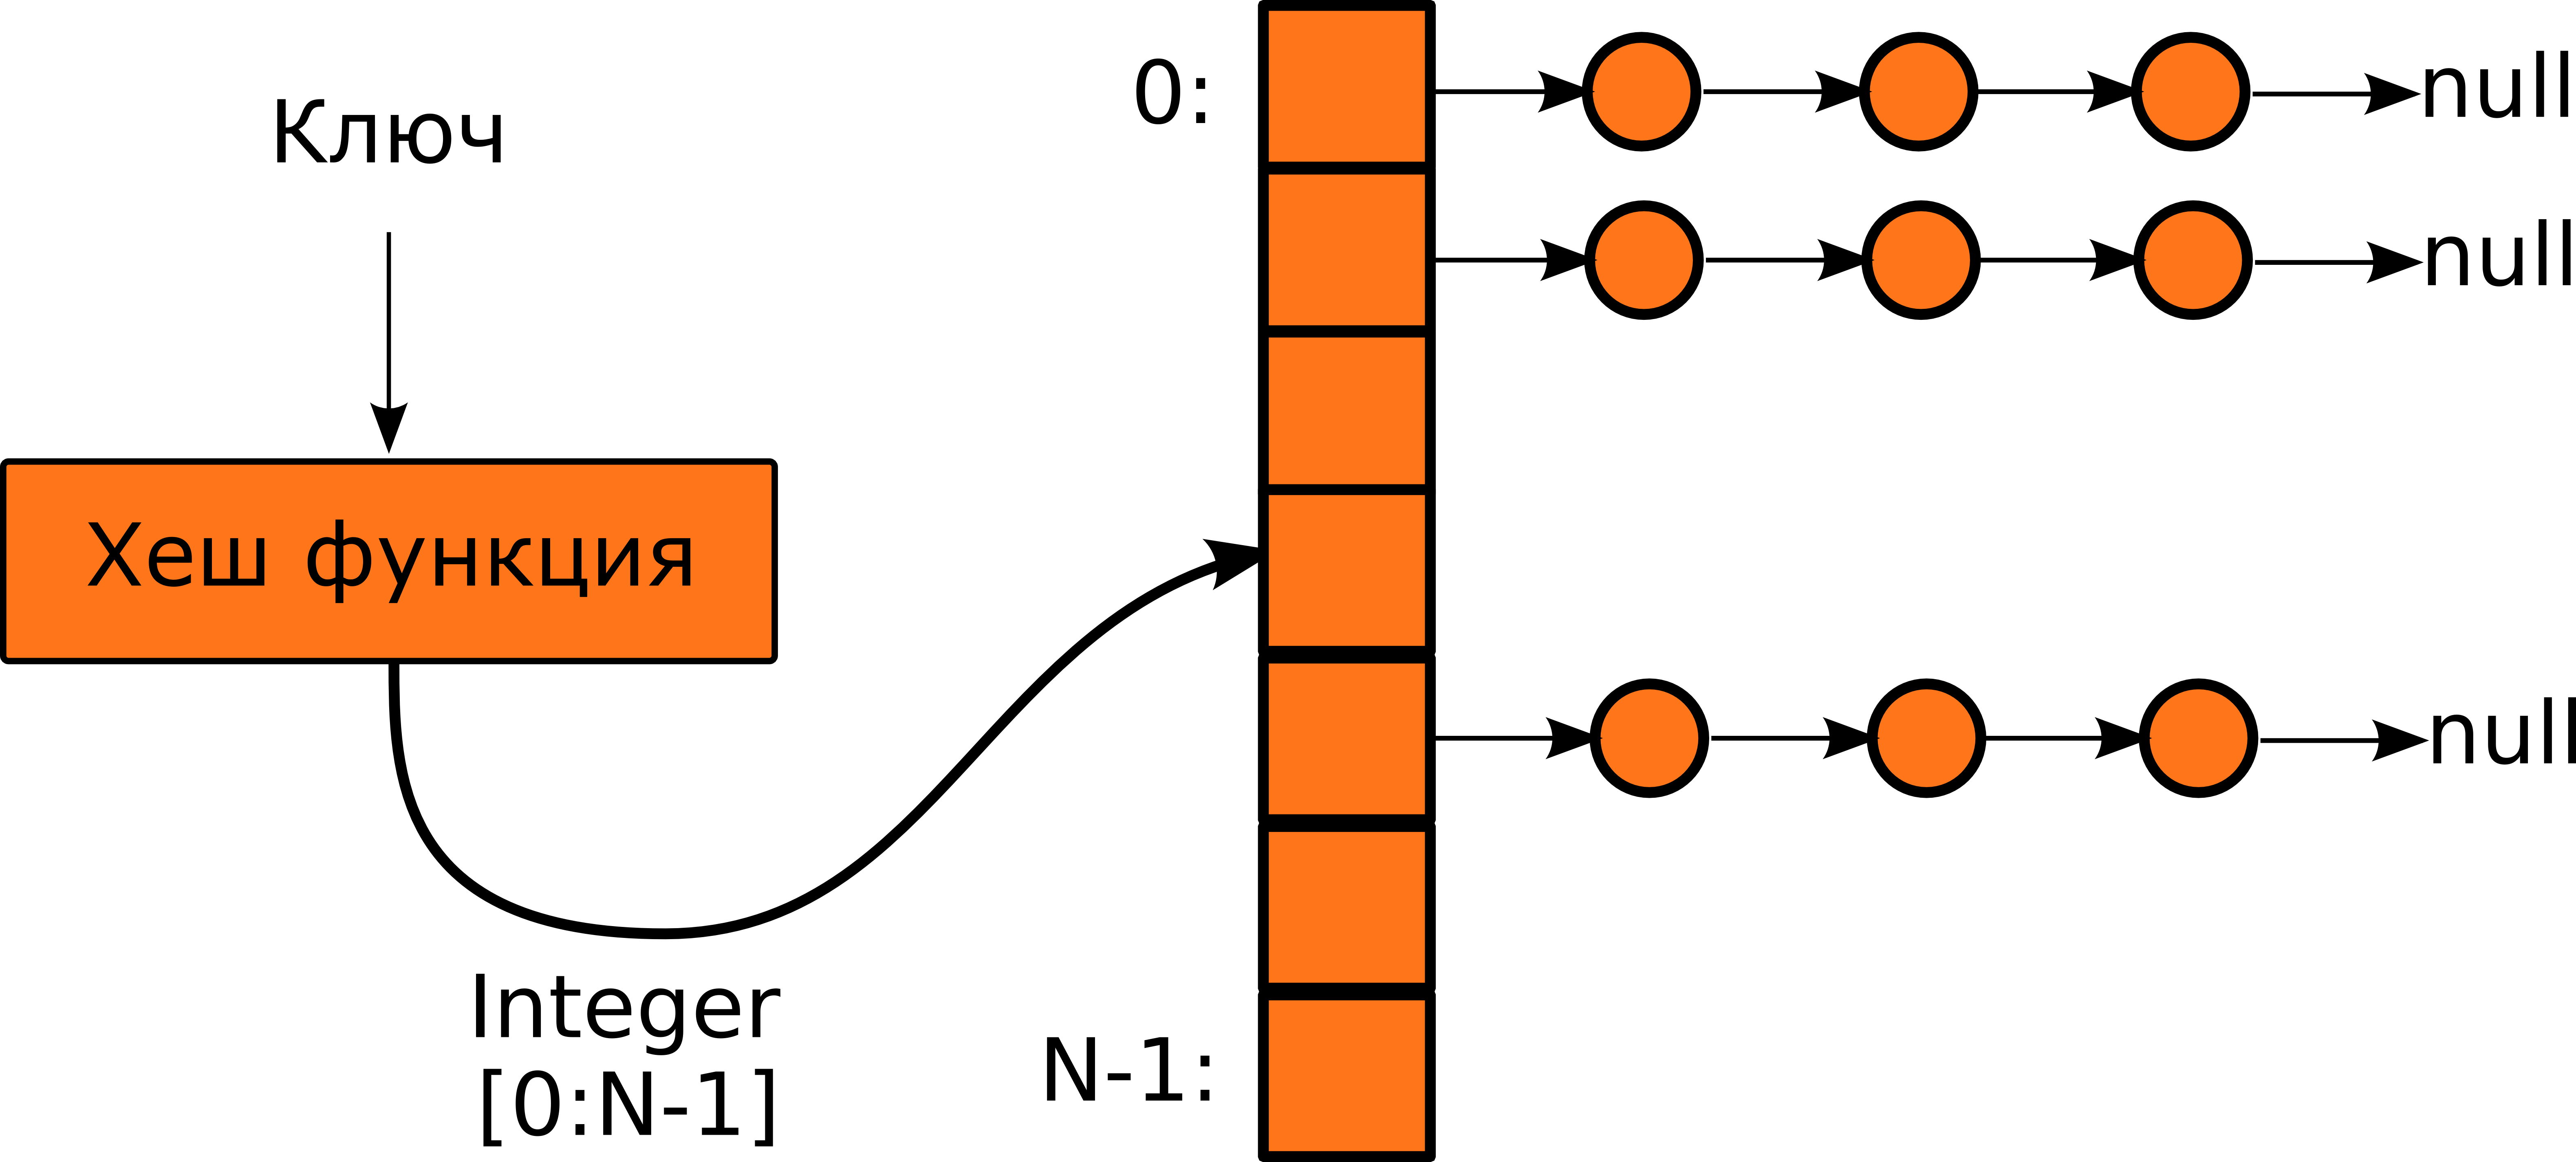
\includegraphics{pics/hash}}
\end{figure}
\end{frame}


\begin{frame}[containsverbatim]\frametitle{Хеш-функция}
\begin{itemize}
 \item Хеш-функцията на обект от даден клас съпоставя цяло число, което се наричат хеш-код
 \item За обектите, които са равни (в смисъла на \lstinline{Object.equals()}), хеш-функцията трябва да дава еднакви хеш-кодове.
 \item Когато хеш-функцията връща различни числа за дадени обекти, то тези обекти задължително трябва да са различни (в смисъл на \lstinline{!Object.equals()}).
\end{itemize}
\end{frame}

\begin{frame}[containsverbatim]\frametitle{Методът \lstinline{hashCode}}
\begin{itemize}
 \item Метод на класа \lstinline{java.lang.Object}, който връща цяло число
 \item Дефиницията на \lstinline{hashCode()} в класа \lstinline{java.lang.Object} връща цяло число, което е практически уникално за дадения екземпляр (на основата на разположението на обекта в паметта).
 \item Всеки клас притежава такъв метод --- или метода, който е наследен от \lstinline{java.lang.Object}, или го предефинира (override)
\end{itemize}
\end{frame}

\begin{frame}[containsverbatim]\frametitle{Изисквания към \lstinline{hashCode}}
\begin{itemize}
 \item Хеш кодът на обекта не трябва да се променя, докато обектът не се променя.
 \item Два обекта, които са равни (в смисъл на \lstinline{equal}), трябва да имат еднакви хеш кодове
 \item Когато два обекта не са равни би било много добре хеш кодове им да не са еднакви
\end{itemize}
\end{frame}

\begin{frame}[containsverbatim]\frametitle{Пример: \lstinline{hashCode}}
\begin{lstlisting}
String scott = "Scotty";
String scott2 = "Scotty";
String corey = "Corey";
System.out.println(scott.hashCode());
System.out.println(scott2.hashCode());
System.out.println(corey.hashCode());
\end{lstlisting}
{\color{blue} -1823897190, -1823897190, 65295514}

\begin{lstlisting}
Integer int1 = 123456789;
Integer int2 = 123456789;
System.out.println(int1.hashCode());
System.out.println(int2.hashCode());
\end{lstlisting}
{\color{blue} 123456789, 123456789}

\end{frame}


\begin{frame}[containsverbatim]\frametitle{Пример: \lstinline{class Name}}
\begin{lstlisting}
public  class Name {
 	public String first;
 	public String last;
 	public Name(String first, String last) {
 		this.first = first;
 		this.last = last;
	}
 	public String toString() {
 		return first + " " + last;
	}
 	public boolean equals(Object o) {
 		return (o instanceof Name &&
 				((Name) o).first.equals(this.first) &&
 				((Name) o).last.equals(this.last));
	}
}
\end{lstlisting}
\end{frame}

\begin{frame}[containsverbatim]\frametitle{Пример: \lstinline{class Name} и \lstinline{hashCode}}
\begin{lstlisting}
Name kyle = new Name("Kyle", "MacLaughlin");
Name jack = new Name("Jack", "Nance");
Name jack2 = new Name("Jack", "Nance");

System.out.println(kyle.equals(jack));
System.out.println(jack.equals(jack2));

System.out.println(kyle.hashCode());
System.out.println(jack.hashCode());
System.out.println(jack2.hashCode());
\end{lstlisting}
{\color{blue} false, true, 6718604, 7122755, 14718739}
\begin{itemize}
\item Обектите \lstinline{jack} и \lstinline{jack2} са равни, но хеш кодовете им са различни.
\end{itemize}
\end{frame}

\begin{frame}[containsverbatim]\frametitle{Наистина ли \lstinline{hashCode} е толкова важна?}
\begin{itemize}
 \item Кодът на класът \lstinline{class Name} изглежда работоспособен
 \item Наистина ли е толкова важно функцията \lstinline{hashCode} да спазва изискванията?
 \item Ако не планираме да използваме функцията \lstinline{hashCode} защо трябва да я предефинираме?
\end{itemize}
\end{frame}

\begin{frame}[containsverbatim]\frametitle{Наистина ли \lstinline{hashCode} е толкова важна?}
\begin{itemize}
 \item Ако не предефинираме метода \lstinline{hashCode} в \lstinline{class Name}, то дефиницията която наследяваме от класа \lstinline{Object} ще противоречи на изискванията към хеш код на обект
 \item Това може да доведе до неочаквани и странни резултати
\end{itemize}
\end{frame}

\begin{frame}[containsverbatim]\frametitle{Неочаквани странни резултати}
\begin{lstlisting}
Set<String> strings = new HashSet<String>();
strings.add("jack");
System.out.println(strings.contains("jack"));

Set<Name> names = new HashSet<Name>();
names.add(new Name("Jack", "Nance"));
System.out.println(names.contains(
				new Name("Jack", "Nance")));
\end{lstlisting}
{\color{blue} true, false}
\end{frame}

\begin{frame}[containsverbatim]\frametitle{Предефиниране на \lstinline{hashCode}}
За да се избегнат неочаквани и странни ефетки е необходимо методът \lstinline{hashCode} да изпълнява следните изисквания:
\begin{itemize}
 \item \lstinline{hashCode} трябва да е еднакъв за обекти, които са равни
 \item \lstinline{hashCode} трябва да не се променя между извиквания на метода при положение, че обектът не се променя.
 \item \lstinline{hashCode} трябва да връща цели числа (\lstinline{int})
 \item препоръчително е \lstinline{hashCode} да връща различни стойности за обекти, които не са равни
\end{itemize}
\end{frame}

\begin{frame}[containsverbatim]\frametitle{Пример: Предефиниране на \lstinline{hashCode}}
\begin{lstlisting}
public class Name {
	...
	public int hashCode() {
 		return 1;
	}
}
\end{lstlisting}
\end{frame}

\begin{frame}[containsverbatim]\frametitle{Пример: Предефиниране на \lstinline{hashCode}}
\begin{lstlisting}
public class Name {
	...
	public int hashCode() {
 		return first.hashCode() + last.hashCode();
	}
}
\end{lstlisting}

\begin{lstlisting}
Set<Name> names = new HashSet<Name>();
names.add(new Name("Jack", "Nance"));
System.out.println(names.contains(
				new Name("Jack", "Nance")));
\end{lstlisting}
{\color{blue} true}
\end{frame}

\begin{frame}[containsverbatim]\frametitle{Пример: Подобрена реализация на \lstinline{hashCode}}
\begin{lstlisting}
public class Name {
	...
	public int hashCode() {
 		return first.hashCode() + 37*last.hashCode();
	}
}
\end{lstlisting}
\begin{itemize}
\item Защо тази реализация е по-добра?
\end{itemize}
\end{frame}

\begin{frame}[containsverbatim]\frametitle{Изисквания към \lstinline{hashCode}}
\begin{itemize}
 \item \lstinline{hashCode} трябва да е еднакъв за обекти, които са равни
 \item \lstinline{hashCode} трябва да не се променя между извиквания на метода при положение, че обектът не се променя.
 \item \lstinline{hashCode} трябва да връща цели числа (\lstinline{int})
 \item {\color{red} препоръчително е \lstinline{hashCode} да връща различни стойности за обекти, които не са равни}
\end{itemize}
\begin{lstlisting}
Name name1=new Name("Jack", "Nance");
Name name2=new Name("Nance","Jack");
\end{lstlisting}
\lstinline{name1.hashCode()!=name2.hashCode()}
\end{frame}

\section{Колекции}

\begin{frame}[containsverbatim]\frametitle{Колекции}
\begin{itemize}
 \item Служат за съхранение и обработка на данни
 \item Съвкупност от класове и интерфейси служещи за:
\begin{itemize}
	\item Добавяне на обекти
	\item Съхранение на обекти
	\item Сортиране на обекти
	\item Обхождане на обекти
	\item Извличане на обекти
\end{itemize}
 \item Предоставят сходен интерфей за достъп до различни реализации на колекции
\end{itemize}
\end{frame}

\begin{frame}[containsverbatim]\frametitle{Пример: Използване на колекции}
\begin{itemize}
 \item Класовете и интерфейсите са дефинирани в групата пакети java.util.*
\end{itemize}
\begin{lstlisting}
package  lab2;

import  java.util.*;

public  class CollectionUser {
 	List<String> list = new ArrayList<String>();
	// ...
 	// ... останалата част от класа
	// ...
}
\end{lstlisting}
\end{frame}

\begin{frame}[containsverbatim]\frametitle{Основни методи на \lstinline{Collection<Foo>}}
\begin{itemize}
 \item \lstinline{boolean add(Foo o)}
 \item \lstinline{boolean contains(Foo o)}
 \item \lstinline{boolean remove(Foo o)}
 \item \lstinline{int size()}
\end{itemize}
\end{frame}

\begin{frame}[containsverbatim]\frametitle{Пример: Използване на колекции}
\begin{lstlisting}
List<Name> nameList = new ArrayList<Name>();

nameList.add(new Name("Laura", "Dern"));
nameList.add(new Name("Toby", "Keeler"));
System.out.println(nameList.size()); 			// => 2

nameList.remove(new Name("Toby", "Keeler"));
System.out.println(nameList.size()); 			// => 1

List<Name> nameList2 = new ArrayList<Name>();
nameList2.add(new Name("Scott", "Ostler"));
nameList.addAll(nameList2);

System.out.println(nameList.size()); 			// => 2
\end{lstlisting}
\end{frame}

\begin{frame}[containsverbatim]\frametitle{Типизирани колекции}
\begin{itemize}
 \item Типизираните колекции предоставят възможност да се укаже явно типът на обектите, които ще бъдат съхранявани в колекцията
\begin{lstlisting}
List<String> stringList;
\end{lstlisting}
 \item По този начин се гарантира, че в колекцията може да има само обекти от даден тип
 \item Не е задължително да се указва типът, но е препоръчително и много удобно
\end{itemize}
\end{frame}

\begin{frame}[containsverbatim]\frametitle{Пример: Използване на типизирани колекции}
\begin{lstlisting}
List untyped = new ArrayList();

Object obj = untyped.get(0);
String sillyString = (String) obj;
\end{lstlisting}
\begin{lstlisting}
List<String> typed = new ArrayList<String>();

String smartString = typed.get(0);
\end{lstlisting}
\end{frame}

\begin{frame}[containsverbatim]\frametitle{Пример: Обхождане на елементите на колекция}
\begin{lstlisting}
Collection<Foo> coll;
...
Iterator<Foo> it = coll.iterator();
while (it.hasNext()) {
	Foo obj = it.next();
	// действия с обекта obj
}
\end{lstlisting}
\begin{lstlisting}
Collection<Foo> coll;
...
for (Foo obj : coll) {
	// действия с обекта obj
}
\end{lstlisting}
\end{frame}

\begin{frame}[containsverbatim]\frametitle{Изтриване на елементи от колекция}
\begin{itemize}
\item Елементи не могат да бъдат изваждани от колекция
докато тя се обхожда. Методът \lstinline{remove()} на колекцията ще генерира изключение {\color{blue}\lstinline{ConcurrentModificationException}}
\begin{lstlisting}
for (Foo obj : coll) {
	coll.remove(obj); // throws
}
\end{lstlisting}
\end{itemize}
\end{frame}

\begin{frame}[containsverbatim]\frametitle{Изтриване на елементи от колекция}
\begin{itemize}
\item Елементите могат да бъдат изтривани от колекция по време на обхождане
посредством итератора:
\begin{lstlisting}
Iterator<Foo> it = coll.iterator();
while (it.hasNext()) {
	Foo obj = it.next();
	it.remove(); // ВМЕСТО coll.remove(obj);
}
\end{lstlisting}
\item Методът remove() не е задължителен и не всеки итератор
 го поддържа. Ако итераторът не притежава този метод, опита да го извикате генерира  {\color{blue}\lstinline{UnsupportedOperationException}}
\end{itemize}
\end{frame}

\begin{frame}[containsverbatim]\frametitle{Основни типове колекция}
\begin{itemize}
\item Списък -- \lstinline{List}, \lstinline{ArrayList}
\item Множество -- \lstinline{Set}, \lstinline{HashSet}, \lstinline{TreeSet}
\item Асоциативен контейнер -- \lstinline{Map}, \lstinline{HashMap}
\end{itemize}
\end{frame}

\begin{frame}[containsverbatim]\frametitle{Списък}
\begin{itemize}
\item Контейнер за данни (съхранява данни)
\item Подредено, линейно множество от елементи
\item Списъкът е динамична колекция -- размерът на списъка е променлива
\item Редът на елементите съвпада с реда на вмъкването им
\end{itemize}
\begin{lstlisting}
List<String> strings = new ArrayList<String>();
strings.add("one");
strings.add("two");
strings.add("three");

// strings = [ “one”, “two”, “three”]
\end{lstlisting}
\end{frame}

\begin{frame}[containsverbatim]\frametitle{Списък: други операции}
\begin{lstlisting}
List<String> strings = new ArrayList<String>();

// Вмъкване след последния елемент
strings.add("one");
strings.add("three");

// Вмъкване на определена позиция
strings.add(1, "two");

// strings = [ “one”, “two”, “three”]

// Достигане до елемент на определена позиция:
System.out.println(strings.get(0)); 		  // => “one”
System.out.println(strings.indexOf("one")); // => 0
\end{lstlisting}
\end{frame}

\begin{frame}[containsverbatim]\frametitle{Множество}
\begin{itemize}
\item Колекция от данни
\item Реализира математическата абстракция множество (set)
\item Редът на вмъкване на елементите не влияе на редът им в множеството
\item Не позволява вмъкването на два еднакви елемента (add() връща false):
\end{itemize}
\begin{lstlisting}
Set<Name> names = new HashSet<Name>();
names.add(new Name("Jack", "Nance"));
names.add(new Name("Jack", "Nance")); 

System.out.println(names.size()); // => 1\end{lstlisting}
\end{frame}

\begin{frame}[containsverbatim]\frametitle{Изисквания към елементите на множеството}
\begin{itemize}
\item След като даден елемент се вмъкне в множеството той не би следвало да бъде ползван по никакъв начин, който би го променило (неговия хеш код и данните за equal())
\item Промяната на елемент от множеството би могло да доведе до неочаквани резултати:
\end{itemize}
\begin{lstlisting}
Set<Name> names = new HashSet<Name>();
Name jack = new Name("Jack", "Nance");
names.add(jack);
System.out.println(names.size()); 			 // => 1
System.out.println(names.contains(jack));// => true;

jack.last = "Vance";

System.out.println(names.contains(jack));// => false
System.out.println(names.size()); 			 // => 1
\end{lstlisting}
\end{frame}

\begin{frame}[containsverbatim]\frametitle{Какво е решението на този проблем?}
\begin{itemize}
\item Няма решение!
\item Единственият начин да се спасите от този проблем е да не променяте състоянието на обекта след като го добавите в някое множество
\item Най-добрият подход е обектите, които се съхраняват в множества или служат за ключове в асоциативни контейнери да бъдат непроменяеми (immutable)
\item Ако все пак се налага да промените състоянието на обект, който е елемент на множество, първо трябва да го изтриете от множеството (за да се избегнат неочаквани резултати) и след като го промените да го добавите отново
\end{itemize}
\end{frame}

\begin{frame}[containsverbatim]\frametitle{Асоциативни контейнери (Map)}
\begin{itemize}
\item Служи за съхранение на връзка между ключ и стойност
\item На всеки ключ съответства стойност
\item Удобно, когато трябва да се осъществи връзка между два обекта и по единия от тях да може бързо да се намери другия
\item Ключовете трябва да са уникални
\item Стойностите не е задължително да са уникални
\end{itemize}
\end{frame}

\begin{frame}[containsverbatim]\frametitle{Асоциативните контейнери не са колекции}
\begin{itemize}
\item Асоциативният контейнер не поддържа методите на колекцията --- \lstinline{boolean add(Foo o)}, \lstinline{boolean contains(Object obj); }
\item Вместо тях асоциатвният контейнер разполага със следните операции:
\begin{lstlisting}
boolean put(Foo key, Bar value);
boolean containsKey(Foo key);
boolean containsValue(Bar value); 
\end{lstlisting}
\end{itemize}
\end{frame}

\begin{frame}[containsverbatim]\frametitle{Използване на асоциативни контейнери}
\begin{itemize}
\item 
\begin{lstlisting}
Map<String, String> dns = 
		new HashMap<String, String>();
\end{lstlisting}
\item Вмъкване на ключ \lstinline{"lubo.elsys-bg.org"} със стойност \lstinline{"82.147.133.129"}
\begin{lstlisting}
dns.put("lubo.elsys-bg.org", 
		"82.147.133.129");

System.out.println(
		dns.get("lubo.elsys-bg.org"));
// => "82.147.133.129"
System.out.println(
		dns.containsKey("lubo.elsys-bg.org"));
// => true
System.out.println(
		dns.containsValue("82.147.133.129"));
// => true
\end{lstlisting}
\end{itemize}
\end{frame}

\begin{frame}[containsverbatim]\frametitle{Използване на асоциативни контейнери}
\begin{itemize}
\item Изтриване на елемент по ключ "lubo.elsys-bg.org"
\begin{lstlisting}
dns.remove("lubo.elsys-bg.org");
System.out.println(
		dns.containsValue("82.147.133.129"));
// => false
\end{lstlisting}
\end{itemize}
\end{frame}

\begin{frame}[containsverbatim]\frametitle{Полезни методи на асоциативен контейнер}
\begin{itemize}
\item \lstinline{keySet()} ---
Връща множество (set, т.е. не може да има повторения) от всички ключове
\item \lstinline{values()} ---
Връща колекция (може да има повторения) от всички стойности
\item \lstinline{entrySet()} ---
Връща множество (set, т.е. не може да има повторения) от двойките ключ-стойност на асоциативния контейнер.
Всяка двойка е обект от тип Map.Entry, който
поддържа методи за достъп до ключа и стойността getKey(), getValue(), setValue()
\end{itemize}
\end{frame}

\begin{frame}[containsverbatim]\frametitle{Проблеми при промяна на ключа}
\begin{itemize}
\item Не трябва да се променя състоянието на обект, който се използва като ключ в асоциативен контейнер
\item Проблемът е напълно аналогичен на разглежданият при множествата
\item Ако ключът бъде променен, ключът и съответстващата му стойност могат да се загубят
\end{itemize}
\end{frame}

\begin{frame}[containsverbatim]\frametitle{Проблеми при промяна на ключа}
\begin{lstlisting}
Name isabella = new Name("Isabella", "Rosellini");
Map<Name, String> directory = 
		new HashMap<Name, String>();
directory.put(isabella, "123-456-7890"); // добавяме
System.out.println(directory.get(isabella));

isabella.first = "Dennis"; // променяме ключа
System.out.println(directory.get(isabella));

// добавяме още един обект със стойност като оригиналния
directory.put(new Name("Isabella", "Rosellini"), 
		"555-555-1234");
// връщаме стойността на оригиналния
isabella.first = "Isabella"; 

System.out.println(directory.get(isabella));
\end{lstlisting}
\end{frame}

\begin{frame}[containsverbatim]\frametitle{Решение чрез копиране на ключа}
\begin{lstlisting}
Name dennis = new Name("Dennis", "Hopper");

// копиране на ключа:
Name copy = new Name(dennis.first, dennis.last);
map.put(copy, "555-555-1234"); // използва се копието

// промяната на dennis не би попречила

// но въпреки това остава опасност от промяна на ключа:
for (Name name : map.keySet()) {
	name.first = "u r wrecked"; // ГРОЗНО!
}
\end{lstlisting}
\end{frame}

\begin{frame}[containsverbatim]\frametitle{Решение чрез непроменяем ключ}
\begin{lstlisting}
public  class Name {
 	public final String first; // т.е. не може да се променя
 	public final String last;

 	public Name(String first, String last) {
 		this.first = first;
 		this.last = last;
	}

 	public boolean equals(Object o) {
 		return (o instanceof Name &&
 				((Name) o).first.equals(this.first) &&
 				((Name) o).last.equals(this.last));
	}
}
\end{lstlisting}
\end{frame}

\begin{frame}[containsverbatim]\frametitle{Решение чрез непроменяем делегат}
\begin{lstlisting}
Map<String, String> dir = 
		new HashMap<String, String>();
Name naomi = new Name("Naomi", "Watts");

String key = naomi.first + "," + naomi.last;
dir.put(key, "888-444-1212");
\end{lstlisting}
\begin{itemize}
\item Обектите от типа \lstinline{String} не могат да бъдат променяни.
\end{itemize}
\end{frame}


\begin{frame}[containsverbatim]\frametitle{Решение чрез замразяване на ключа}
\begin{lstlisting}
public  class Name {
 	private String first;
 	private String last;
 	private boolean frozen = false; 

 	public void setFirst(String s) {
 		if (!frozen) 
 			first = s;
	}
 	// аналогично за setLast()

 	// „замразяваме“ обекта
 	public void freeze() {
 		frozen = true;
	}
}
\end{lstlisting}
\end{frame}

\begin{frame}[containsverbatim]\frametitle{Променяеми ключове}
\begin{itemize}
\item Всеки подход за решавне на проблемът с променяемите ключове има своите предимства и недостатъци
\item Винаги използвайте възможно най-простото решение, което е подходящо за ситуацията
\item Ако ключът не може да се променя, то няма да имате никакви проблеми
\end{itemize}
\end{frame}


\begin{frame}[containsverbatim]\frametitle{Чести грешки при работа с колекции}
\begin{itemize}
\item Изтриване на елемент от списък докато го обхождаме
\item Промяна на елемент в множество
\item Промяна на ключ в асоциативен контейнер
\end{itemize}
\end{frame}

\section{Сравняване и сортиране}

\begin{frame}[containsverbatim]\frametitle{Сравняване и сортиране}
\begin{itemize}
\item Използва се за да се прецени кой от два обекта е по-голям или двата обекта са равни
\item Изразът \lstinline{a.compareTo(b)} връща следните стойности:
\begin{itemize}
\item \lstinline{<0} ако \lstinline{a<b}
\item \lstinline{==0} ако \lstinline{a==b}
\item \lstinline{>0} ако \lstinline{a>b}
\end{itemize}
\end{itemize}
\end{frame}

\begin{frame}[containsverbatim]\frametitle{Пример: Сравнения}
\begin{lstlisting}
Integer one = 1;
System.out.println(one.compareTo(3)); 		// => -1
System.out.println(one.compareTo(-50)); 	// => 1

String frank = "Frank";
System.out.println(frank.compareTo("Booth"));  // => 4
System.out.println(frank.compareTo("Hopper")); // => -2
\end{lstlisting}
\end{frame}

\begin{frame}[containsverbatim]\frametitle{Пример: Азбучно сортиране на списък}
\begin{lstlisting}
List<String> names = new ArrayList<String>();
// добавяне на елементи към списъка
names.add("Sailor");
names.add("Lula");
names.add("Bobby");
names.add("Santos");
names.add("Dell");

// сортиране на списъка
Collections.sort(names);
	
// names => [ "Bobby", "Dell", "Lula", "Sailor", "Santos" ]
\end{lstlisting}
\end{frame}

\begin{frame}[containsverbatim]\frametitle{Интерфейсът \lstinline{Comparable}}
\begin{itemize}
\item За да се сортират елементите на списъка трябва да имплементират интерфейса Comparable
\item Методът, който трябва да бъде реализиран е:
\begin{lstlisting}
int compareTo(Object obj); 
\end{lstlisting}
\item Класът \lstinline{String} имплементира интерфейсът \lstinline{Comparable} и поради това списък от низове може да бъде сортиран
\end{itemize}
\end{frame}

\begin{frame}[containsverbatim]\frametitle{Пример: Сортиране на класът \lstinline{Name}}
\begin{lstlisting}
public  class Name implements Comparable<Name> {
	// ...

 	// сортиране по фамилия
 	public int compareTo(Name o) {
 		int compare = this.last.compareTo(o.last);
 		if (compare != 0)
 			return compare;
 		else
 			return this.first.compareTo(o.first);
	}
}
\end{lstlisting}
\end{frame}

\begin{frame}[containsverbatim]\frametitle{Пример: Сортиране на класът \lstinline{Name}}
\begin{lstlisting}
List<Name> names = new ArrayList<Name>();
names.add(new Name("Nicolas", "Cage"));
names.add(new Name("Laura", "Dern"));
names.add(new Name("Harry", "Stanton"));
names.add(new Name("Diane", "Ladd"));
names.add(new Name("William", "Morgan"));
names.add(new Name("Dirty", "Glover"));
names.add(new Name("Johnny", "Cage"));
names.add(new Name("Metal", "Cage"));

System.out.println(names);
Collections.sort(names);
System.out.println(names);

// => [Johnny Cage, Metal Cage, Nicolas Cage, Laura Dern,
//  Crispin Glover,Diane Ladd, William Morgan, Harry Stanton]
\end{lstlisting}
\end{frame}

\begin{frame}[containsverbatim]\frametitle{Интерфейсът \lstinline{Comparator}}
\begin{itemize}
\item Позволява едни и същи данни да бъдат сортирани по различни критерии
\item Сравнява два обекта
\item Методът, който трябва да се реализира е:
\begin{lstlisting}
int compare(Object o1, Object o2); 
\end{lstlisting}
\end{itemize}
\end{frame}


\begin{frame}[containsverbatim]\frametitle{Пример: Сортиране на класът \lstinline{Name} по първо име}
\begin{lstlisting}
import java.util.Comparator;

public class FirstNameFirst 
			implements Comparator<Name> {
 	//сортиране по първо име
 	public int compare(Name n1, Name n2) {
 		int ret = n1.first.compareTo(n2.first);
 		if (ret != 0)
 			return ret;
 		else
 			return n1.last.compareTo(n2.last);
	}
}
\end{lstlisting}
\end{frame}

\begin{frame}[containsverbatim]\frametitle{Пример: Сортиране на класът \lstinline{Name} по първо име}
\begin{lstlisting}
List<Name> names = new ArrayList<Name>();
// ...

// създаваме обект, чрез който ще
// извършваме сравненията по време на сортиране
Comparator<Name> first = new FirstNameFirst();
Collections.sort(names, first);

System.out.println(names);

// => [Crispin Glover, Diane Ladd, Harry Stanton, JohnnyCage, 
// Laura Dern, Metal Cage, Nicolas Cage, WilliamMorgan]
\end{lstlisting}
\end{frame}

\begin{frame}[containsverbatim]\frametitle{Изисквания към сравняване}
\begin{itemize}
\item Резултатът при сравнението на два обекта винаги не трябва да се променя (ако обектите не се променят)!
\item Особено внимание трябва да се обръща на ситуациите \lstinline{(compare(e1, e2)==0) != e1.equals(e2)}. Такива ситуации трябва да се избягват.
\item Такива случаи биха довели до неопределени резултати при сортирането на колекции като \lstinline{SortedSet}, \lstinline{SortedMap} и т.н.
\end{itemize}
\end{frame}

\begin{frame}[containsverbatim]\frametitle{Сортирани множества}
\begin{itemize}
\item Ако искаме елементите в множеството да бъдат сортирани, можем да използваме имплементацията \lstinline{TreeSet}.
\item Елементите на множеството \lstinline{TreeSet} трябва да имплементират интрефейсът \lstinline{Comparable} или при създаване на множеството \lstinline{TreeSet} трябва да подадете допълнителен обект, който имплементира интерфейсът \lstinline{Comparator}
\end{itemize}
\begin{lstlisting}
SortedSet<Name> names = new TreeSet<Name>(
			new FirstNameFirst());
names.add(new Name("Laura", "Dern"));
names.add(new Name("Harry", "Stanton"));
names.add(new Name("Diane", "Ladd"));

System.out.println(names);
// => [Diane Ladd, Harry Stanton, Laura Dern]
\end{lstlisting}
\end{frame}


\end{document}
